\chapter{Introduction}
\label{ch:introduction}

\dictum[George Box]{%
  All models are wrong, but some are useful.}%
\vskip 1em

\chapterabstract{
   Abstract comes here
}

\section{How to use this template}

Citations work as usual,\cite{Maxwell1865} or like Ref. \citenum{Maxwell1865}. 

%
Equations look like this
%
\begin{align}
    i\hbar\frac{\d }{\d t}\ket{\Psi(\bm{r},t)} =   \hat{\mathpzc{H}}\ket{\Psi(\bm{r},t)}
    \label{eq:tdse}
\end{align}
%

\subsection{Figures and tables}

\lipsum[1-3]


\begin{figure}[t!]
    \centering
    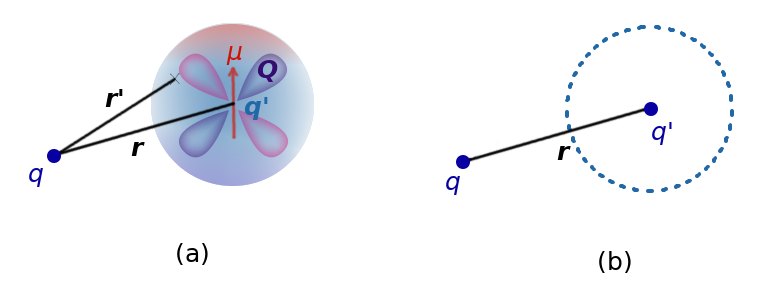
\includegraphics[width=0.9\textwidth]{chapters/introduction/figures/multipole.png}
    \caption{Figures are to be top-aligned wherever possible.}
    \label{fig:intro-multipole}
\end{figure}

\lipsum[4-6]

%
\begingroup
\rowcolors{2}{\tabcol!25}{\tabcol!5}

\begin{table}[t!]
	\centering
	\caption{
%
Note the \texttt{rowcolor} statements in the table to adjust the colors. Cannot be set for the whole document as some math environments are internally tables.
%
%
}
	\begin{tabular}{c | c  c  c }
	\rowcolor{\tabcol!50}
		    & option A & option B & option C \\
		1 & -5807.4 & 5.18 & 20.677 \\
		2 & -5807.4 & 0.65 & 20.714 \\
		3 & -5807.2 & 0.21 & 20.801 \\
		4 & -5807.2 & 0.09 & 20.959 \\
		5 & -5807.3 & 0.04 & 21.204 \\
	\end{tabular}
	\label{tab:hom-utot}
\end{table}
\endgroup
%
